\section{Руководство пользователя}
\label{sec:guide}

Данное программное обеспечение призвано для упрощения процесса проведения функционального ТС КМУ артиллерийского
дивизиона.\break
Программное обеспечение используется в составе комплекса программ для автоматизации АРМ.
Комплекс программ устанавливается на все АРМ КМУ артиллерийского дивизиона.

В данном разделе приведено рукводство оператора АРМ по использованию системы функционального контроля.
Руководство включает в себя требования к аппаратному и программному обеспечению, последовательность запуска, выполнения
и завершение программы функционального контроля, а также приведены сообщения, возникающие при функционировании программы
с указанием возможных команд по управлению процессом выполнения программы.

\subsection{Требования к аппаратному и программному обеспечению}
\label{sub:guide:reqs}

Так как разработанное ПО используется в составе комплекса программ для автоматизации АРМ, ниже приведены требования к
аппаратному и программному обеспечению для работы всего программного комплекса.

Программный комплекс устанавливается на ПЭВМ и бортовую ЭВМ.

ПЭВМ должна иметь следующие характеристики:
\begin{itemize}
	\item центральный процессор -- Intel Pentium с частотой не менее 1,90 ГГц;
	\item объем оперативной памяти -- 4 ГБ;
	\item объем накопителя на жестком диске, SSD -- не менее 256 ГБ;
	\item сетевой адаптер -- Ethernet 10/100/1000 Мбит/с;
	\item порт USB 2.0 -- 2 шт.;
	\item порт RS232/422/485 -- 4 шт.;
	\item порт DVI -- 1 шт.
\end{itemize}

Бортовая ЭВМ должна иметь следующие характеристики:
\begin{itemize}
	\item центральный процессор -- Intel с частотой не менее 1.6 ГГц;
	\item объем оперативной памяти -- не менее 4 ГБ;
	\item сенсорный экран -- размер не менее 10 дюймов (разрешение не менее 1280х800);
	\item объем накопителя на жестком диске, SSD -- не менее 240 ГБ;
	\item сетевой адаптер -- Ethernet 10/100/1000 Мбит/с не менее 2 шт.;
	\item порт USB 2.0 -- не менее 2 шт.;
	\item порт RS232 -- не менее 1 шт.
\end{itemize}

Для загрузки ПО требуется внешний привод DVD-ROM с возможностью подключения к порту USB.
В меню настроек BIOS компьютеров первым устройством должно быть установлено устройство чтения DVD -- ROM.
Программа функционального контроля функционирует в сети ETHERNET с пропускной способностью 10/100/1000 Мбит/с.
Дополнительно для функционирования ПЭВМ должно быть установлено следующее периферийное оборудование:

\begin{itemize}
	\item принтер промышленный;
	\item видеомонитор;
	\item клавиатура;
	\item манипулятор графической информации (МГИ).
\end{itemize}

Для функционирования программы фукнционального контроля должна быть установлена 64-разрядная
операционная система Windows 7\break Professional или Windows 7 Ultra.

\subsection{Установка программного обеспечения}
\label{sub:guide:intstallation}

Данное ПО предназначено для использования в составе программного комплекса по автоматизации АРМ КМУ
артиллерийского дивизиона.
Установка программного комплекса на ЭВМ КМУ артиллерийского дивизиона в данном разделе
рассмотрена не будет.

Для использования в тестовых и демонстрационных целях система\break функционального контроля может быть установлена и
использоваться отдельно от остального комплекса.
В этом случае для установки достаточно скопировать содержимое диска
с ПО на компьютер.

\subsection{Руководство по использованию системы}
\label{sub:guide:user_guide}

При использовании системы в составе программного комплекса, запуск программы осуществляется с помощью соответствеющих
элементов графического интерфейса главного окна управляющей программы комплекса.

Запуск программы тестирования устройств
осущетвляется запуском\break файла OfflinefunctionControl.exe, который находится в
подкаталоге bin каталога системы функционального контроля.
В результате запуска программы отобразится главное окно <<Функциональный контроль>> программы, приведенное на рис.
\ref{fig:guide:user_guide:main_window}.
\begin{figure}[ht]
	\centering
	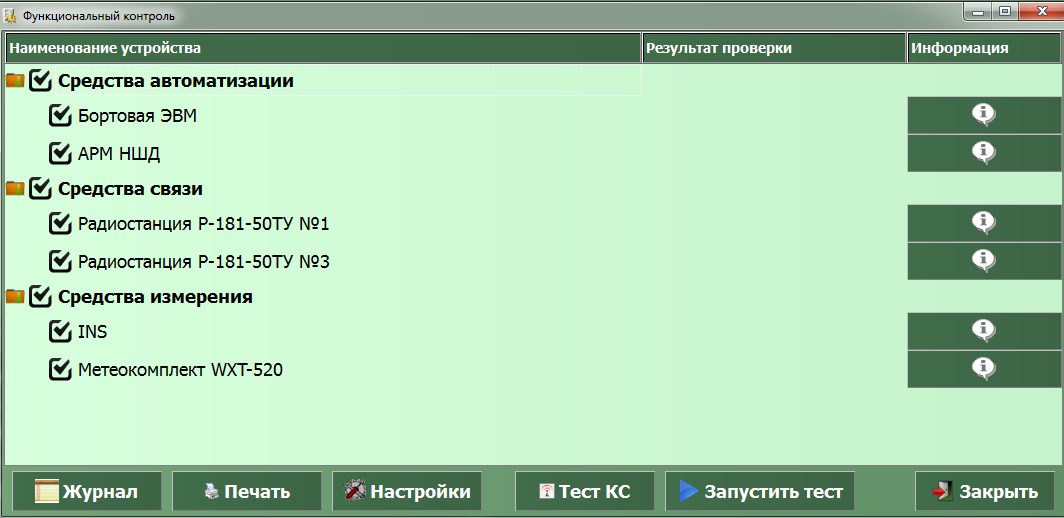
\includegraphics[scale=0.35]{main_window}
	\caption{Окно <<Функциональный контроль>>}
	\label{fig:guide:user_guide:main_window}
\end{figure}

Окно <<Функциональный контроль>> содержит список тестируемых технических средств
(наименование и количество устройств могут изменяться в зависимости от настроек АРМ).
Слева от наименования устройства имеется поле для установки флажка.
При нажатии кнопки <<Запустить тест>> запускаются тесты, отмеченные флажками.
При установке (снятии) флажка <<Средства автоматизации>>, <<Средства связи>>,
<<Средства измерения>> автоматически
устанавливаются (снимаются) флажки всех устройств, входящих в эту группу.
Тесты могут запускаться как по одному, так и все одновременно.
Результаты тестирования отображаются в столбце <<Результат проверки>> в виде сообщений:
\begin{itemize}
		\item <<Исправно>> (зеленого цвета);
		\item <<Неисправно>> (красного цвета);
		\item <<Порт занят>> (красного цвета).
\end{itemize}

При нажатии кнопки в столбце <<Информация>> открывается окно с подробной информацией о результатах проверки,
например, <<Бортовая ЭВМ>> (рис. \ref{fig:guide:user_guide:on_info}).
\begin{figure}[ht]
	\centering
	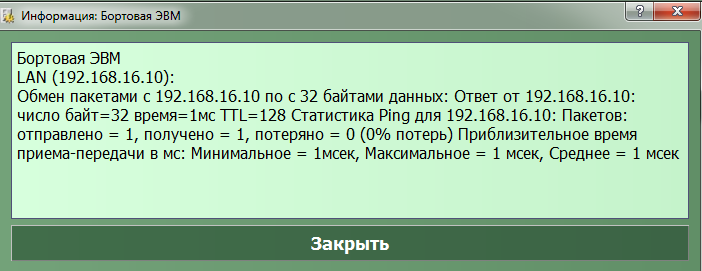
\includegraphics[scale=0.40]{on_info}
	\caption{Окно <<Информация: Бортовая ЭВМ>>}
	\label{fig:guide:user_guide:on_info}
\end{figure}
Для выхода из окна <<Информация: Бортовая ЭВМ>> нажать кнопку <<Закрыть>>.

Для тестирования каналов обмена данными необходимо нажать кнопку <<Тест КС>> (см. рис.
\ref{fig:guide:user_guide:main_window}).
В результате выполнения команды отобразится окно <<Тест каналов связи по радиостанциям Р–180/181>>, приведенное на рис.
\ref{fig:guide:user_guide:on_test_cs}.
\begin{figure}[ht]
	\centering
	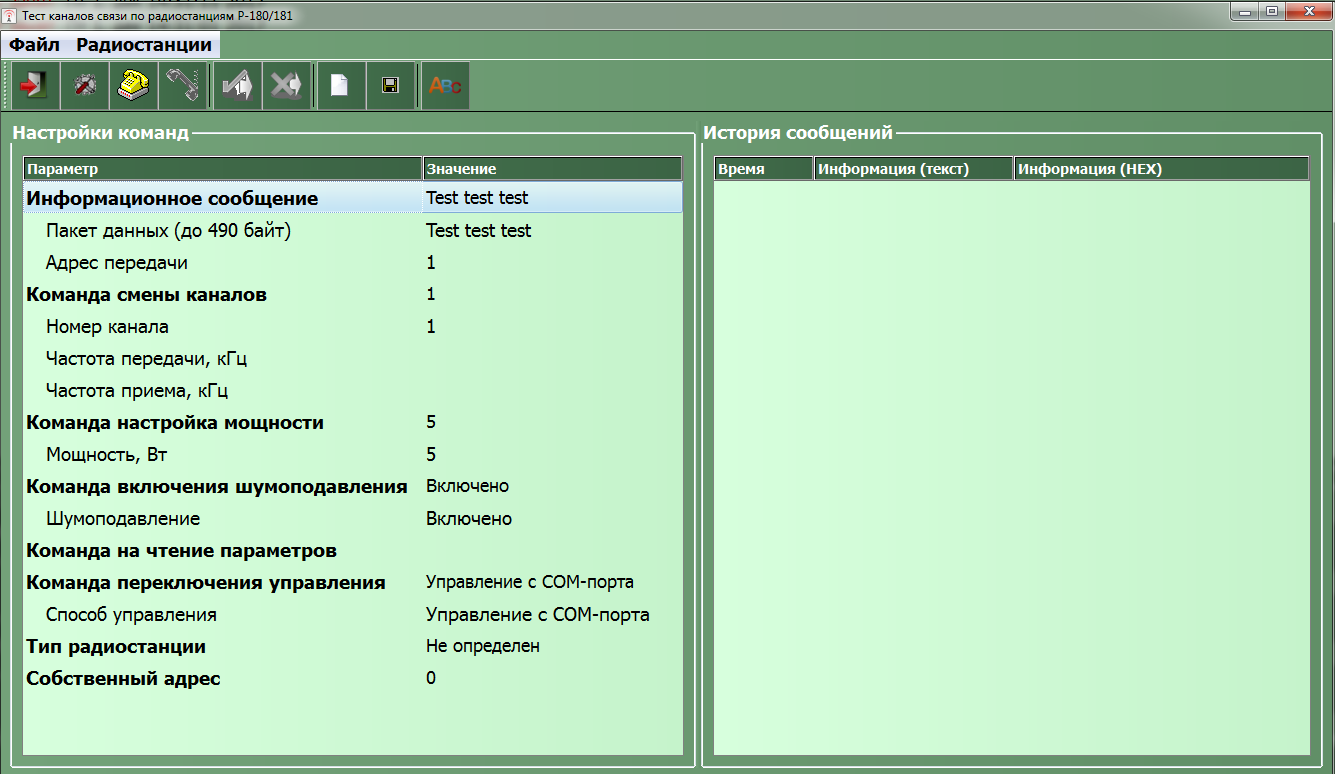
\includegraphics[scale=0.30]{on_test_cs}
	\caption{Окно <<Тест каналов связи по радиостанциям Р–180/181>>}
	\label{fig:guide:user_guide:on_test_cs}
\end{figure}
В левой части окна (см. рис. \ref{fig:guide:user_guide:on_test_cs}) отображается таблица <<Настройки команд>> с параметрами и значениями команд.
В правой части окна отображается таблица <<История сообщений>>, в которой хранится время получения сообщения.
В верхней части окна находится панель инструментов с кнопками, предназначенными для вызова требуемых функций.

Cлева направо на панели инструментов (см. рис. \ref{fig:guide:user_guide:on_test_cs}) расположены\break кнопки: <<Выход>>,
<<Настройки>>, <<Открыть порт>>, <<Закрыть порт>>,
<<Отправить сообщение>>, <<Очистить историю сообщений>>,
<<Сохранить историю сообщений>>, <<Режим ввода>>.

В меню <<Файл>> могут выполняться следующие команды:
\begin{itemize}
	\item <<Настройки>>;
	\item <<Открыть порт>>;
	\item <<Закрыть порт>>;
	\item <<Показать историю сообщений>>;
	\item <<Сохранить историю сообщений>>;
	\item <<Выход>>.
\end{itemize}
Команды меню <<Файл>> дублируют кнопки панели инструментов.

Для настройки порта нажать кнопку <<Настройки>> на панели инструментов (см. рис. \ref{fig:guide:user_guide:on_test_cs}) или выполнить команду
<<Настройки>> из меню <<Файл>>.
В результате выполнения команды отобразится окно, приведенное на рис. \ref{fig:guide:user_guide:port_config}.
\begin{figure}[ht]
	\centering
	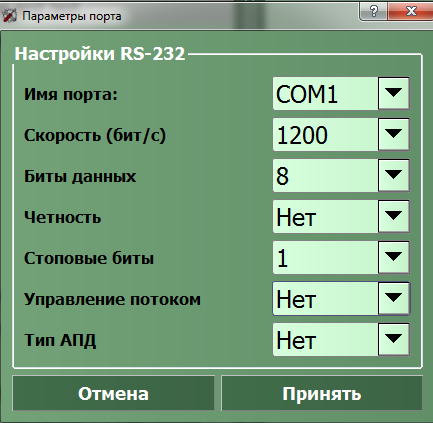
\includegraphics[scale=0.35]{port_config}
	\caption{Настройка параметров порта}
	\label{fig:guide:user_guide:port_config}
\end{figure}
Для проверки канала связи необходимо выдать информационное сообщение, для чего нажать кнопку <<Отправить сообщение>> на
панели инструментов окна <<Тест каналов связи по радиостанциям Р–180/181>> (см. рис.
\ref{fig:guide:user_guide:on_test_cs}) или выполнить команду <<Отправить сообщение>> из контекстного меню.
Переданное сообщение отображается в таблице <<История сообщений>>, в которой отображаются и полученные сообщения от абонента.

По нажатию кнопки <<Печать>> в окне <<Функциональный контроль>>
(см. рис. \ref{fig:guide:user_guide:main_window}) формируется для просмотра и выдачи на принтер отчет
о проведенном функциональном контроле (рис. \ref{fig:guide:user_guide:on_print}).
\begin{figure}[ht]
	\centering
	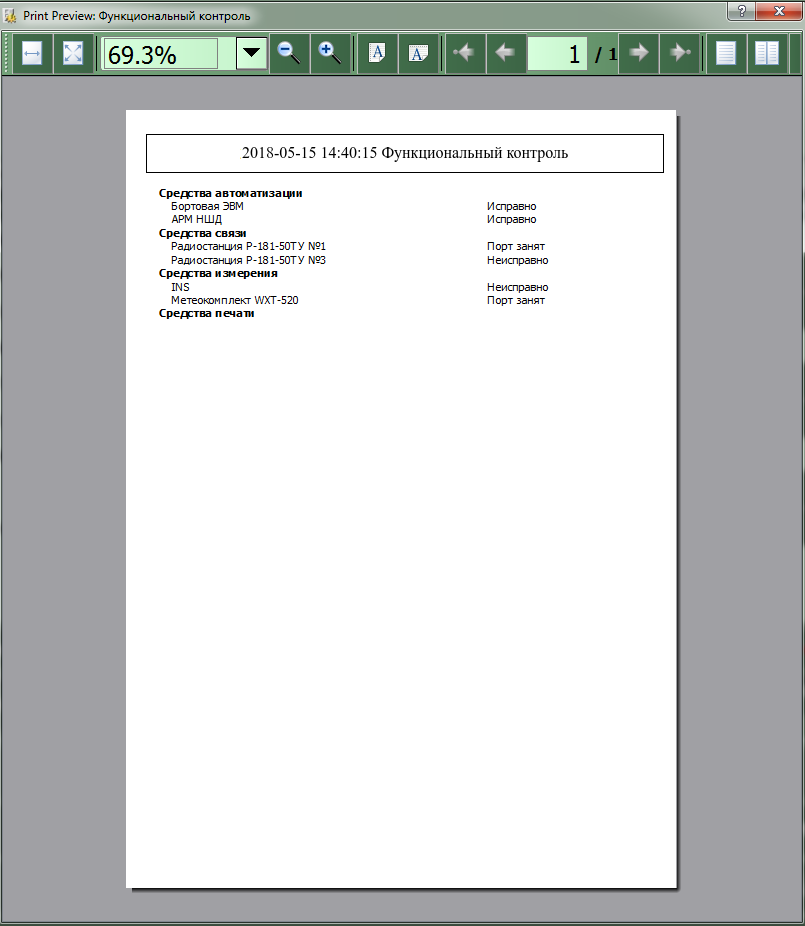
\includegraphics[scale=0.30]{on_print}
	\caption{Окно предварительного просмотра отчета перед печатью}
	\label{fig:guide:user_guide:on_print}
\end{figure}

Программа <<Настройка навигационной системы>> предназначена для настройки бесплатформенной инерциальной навигационной системы БИНС-3.
Для запуска данной системы необходимо запустить файл VSettBINS3.exe.
В результате вызова функции отобразится окно <<Настройка навигационной системы INS>>, приведенное на рис.
\ref{fig:guide:user_guide:ins_window}.
\begin{figure}[ht]
	\centering
	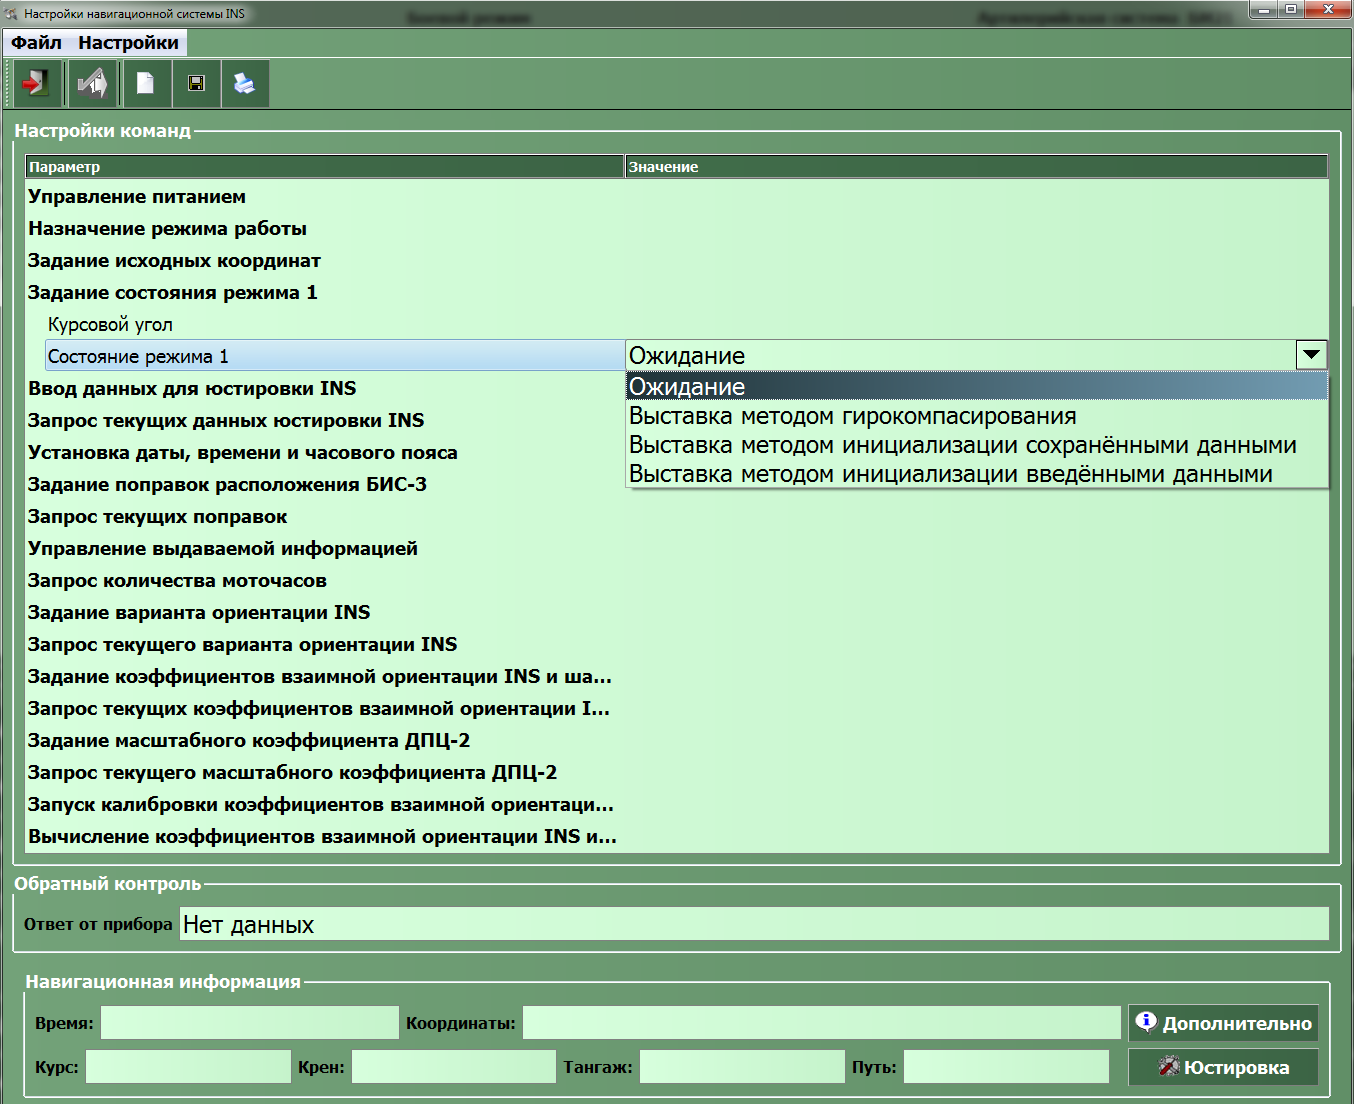
\includegraphics[scale=0.22]{ins_window}
	\caption{Настройка навигационной системы INS}
	\label{fig:guide:user_guide:ins_window}
\end{figure}
В группе <<Навигационная информация>> в полях <<Время>>, <<Координаты>>, <<Курс>>, <<Крен>>, <<Тангаж>>, <<Путь>> спустя некоторое
время после включения будут
отображаться соответствующие данные, полученные в навигационном сообщении от БИНС-3.

При нажатии кнопки <<Юстировка>> (см. рис. \ref{fig:guide:user_guide:ins_window}) отобразится окно для ввода данных,
необходимых при юстировке БИНС-3 (рис. \ref{fig:guide:user_guide:ust}).
Поля <<Курсовой угол>>, <<Крен>>, <<Тангаж>> - редактируемые числовые поля.
После завершения работ по юстировке БИНС-3 закрытие окна осуществляется нажатием на кнопку <<Закрыть>>.
\begin{figure}[ht]
	\centering
	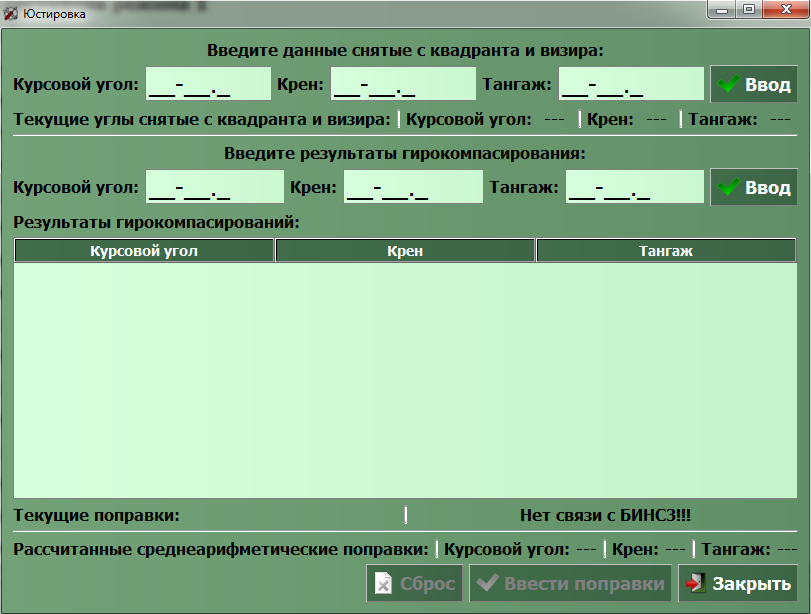
\includegraphics[scale=0.35]{ust}
	\caption{Окно <<Юстировка>>}
	\label{fig:guide:user_guide:ust}
\end{figure}
Для выхода из окна <<Настройка навигационной системы INS>> нажать кнопку <<Выход>> на панели инструментов
или выполнить команду <<Выход>> из меню <<Файл>> (см. рис. \ref{fig:guide:user_guide:ins_window}).

Программа <<Настройка метеостанции WXT-520>> предназначена для настройки настройки метеостанции.
Для запуска данной системы необходимо запустить файл VSetMeteoWXT520.exe.
В результате вызова функции отобразится окно <<Настройка метеостанции WXT-520>>, приведенное на рис.
\ref{fig:guide:user_guide:meteo_window}.
\begin{figure}[ht]
	\centering
	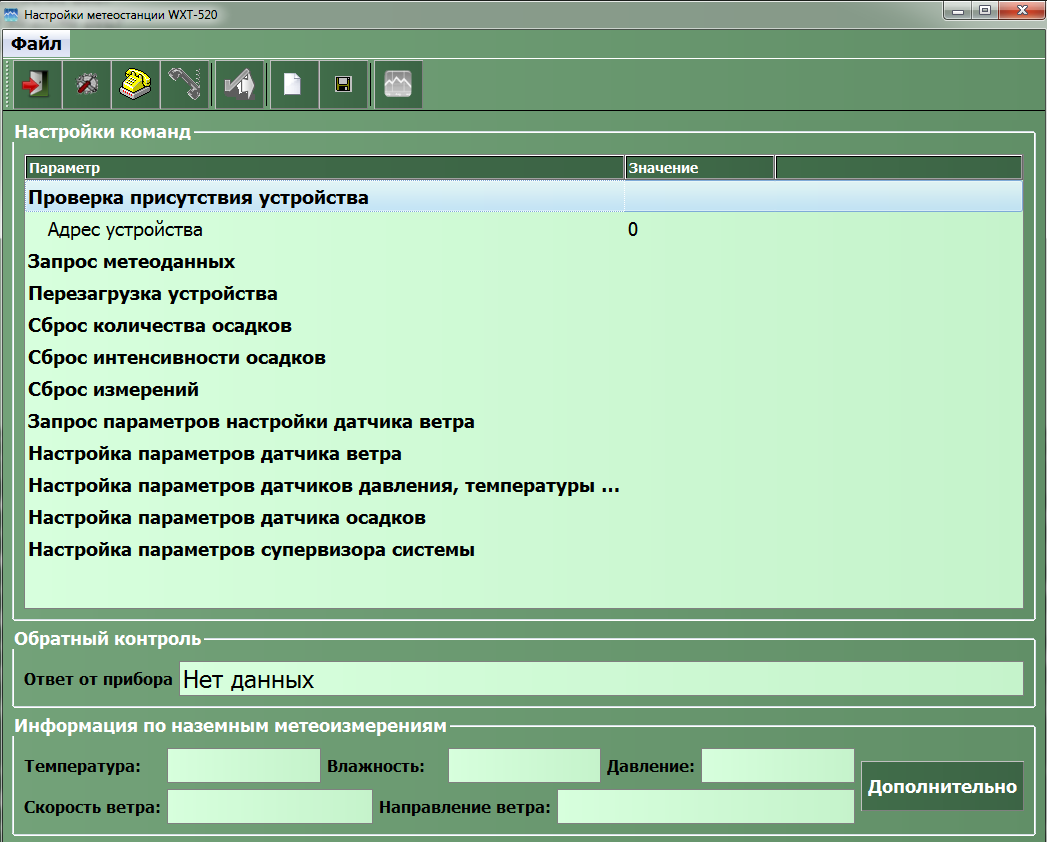
\includegraphics[scale=0.35]{meteo_window}
	\caption{Настройка метеостанции}
	\label{fig:guide:user_guide:meteo_window}
\end{figure}
Если от метеостанции получен ответ, то в поле <<Ответ от прибора>> будет отображаться информация <<Активна>>.

Cлева направо на панели инструментов (см. рис. \ref{fig:guide:user_guide:meteo_window}) расположены\break кнопки: <<Выход>>,
<<Настройки>>, <<Открыть порт>>, <<Закрыть порт>>, <<Отправить сообщение>>, <<Очистить историю сообщений>>,
<<Сохранить историю сообщений>>, <<Сценарий автоматической настройки>>.

В меню <<Файл>> могут выполняться следующие команды:
\begin{itemize}
	\item <<Настройки>>;
	\item <<Открыть порт>>;
	\item <<Основные команды>>;
	\item <<Закрыть порт>>;
	\item <<Полный перечень команд>>;
	\item <<Показать историю сообщений>>;
	\item <<Сохранить историю сообщений>>;
	\item <<Выход>>.
\end{itemize}
Для отправки выбранной команды (по усмотрению оператора) необходимо нажать кнопку <<Отправить сообщение>> на панели инструментов, либо выбрать команду
<<Отправить сообщение>> из контекстного меню. В строке <<Ответ от прибора>> появится ответная информация на выданную команду.
Текущая принятая информация с данными наземных метеоизмерений отображается в соответствующих строках: <<Температура>>,
<<Влажность>>, <<Давление>>, <<Скорость ветра>>, <<Направление ветра>>.
